\documentclass{article}
\usepackage{graphicx}
\usepackage{subcaption}
\begin{document}
Compose a program to multiply two NxN matrices in C.\\
See "matrixTemplate.c" and "matrixTemplate.h". It's a function template other than a complete program.\\

Create a script to generate six programs that will multiple the same matrices with identical data in six different (i,j,k) orders.\\
See "program\_generator.py". I wrote a Python script to generate the six function of different (i,j,k) orders.\\

Verify that the outputs of six different matrix programs are identical.\\
There is an int type varibale \texttt{check} in the "main.c". The program will compare the result of the six functions if \texttt{check} is set to 1.\\

Compose a script to harvest the running times of N=100, 500, 1000 for the six different programs.\\
There is a const int type varibale \texttt{N} defines the size of the matrix in the "main.c". The main function will run the six matrix multiplication functions. I simply change the varibale and ran the program for the three N values.\\

Plot your results with explanations. There are two investigations: a) performance behavior for six orders, and b) performance behavior for different N.\\
    \begin{figure}[h!]
        \centering
        \begin{subfigure}[b]{0.4\linewidth}
          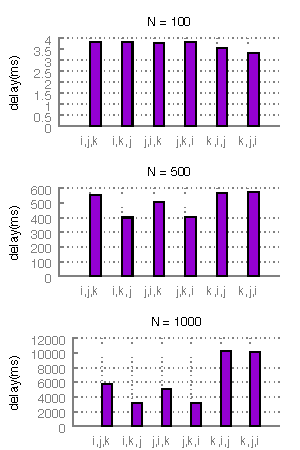
\includegraphics[width=\linewidth]{matrix_ijk.pdf}
          \caption{different i-j-k order}
        \end{subfigure}
        \begin{subfigure}[b]{0.4\linewidth}
          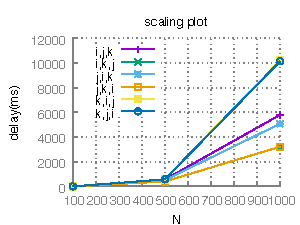
\includegraphics[width=\linewidth]{matrix_scaling.pdf}
          \caption{Scaling}
        \end{subfigure}
        \caption{The same cup of coffee. Two times.}
        \label{fig:coffee}
    \end{figure}
\end{document}